\documentclass[letterpaper,11pt]{article}
\usepackage{natbib}
\bibliographystyle{unsrtnat}
\usepackage{tabularx} % extra features for tabular environment
\usepackage{amsmath}
\usepackage{amssymb}
\usepackage{amsfonts}
\usepackage{mathtools}
\usepackage{tikz}
\usepackage{graphicx} % takes care of graphic including machinery
\usepackage[margin=1in,letterpaper]{geometry} % decreases margins
%\usepackage{cite} % takes care of citations
\usepackage[final]{hyperref} % adds hyper links inside the generated pdf file
\graphicspath{ {./images/} }

\DeclarePairedDelimiter\floor{\lfloor}{\rfloor}  % improve math presentation
\hypersetup{
	colorlinks=true,       % false: boxed links; true: colored links
	linkcolor=blue,        % color of internal links
	citecolor=blue,        % color of links to bibliography
	filecolor=magenta,     % color of file links
	urlcolor=blue         
}
%+++++++++++++++++++++++++++++++++++++++

\begin{document}

\title{Discrete Math Question Set 5}
\author{Abrar Habib}
\date{December 22, 2022}
\maketitle

\begin{enumerate}
    \item A chain letter starts with a person sending a letter out to 10 others. Each person is asked to send the letter
    out to 10 others, and each letter contains a list of the previous six people in the chain. Unless there are fewer
    than six names in the list, each person sends one dollar to the first person in this list, removes the name of this
    person from the list, moves up each of the other five names one position, and inserts his or her name at the
    end of this list. If no person breaks the chain and no one receives more than one letter, how much money will
    a person in the chain ultimately receive?
    \item [] Each person introduces to 10 other people, so we get $10\cdot 10\cdot 10\cdot 10\cdot 10\cdot 10 = 10^6 = 1,000,000$ The first person on the list is on everyone else's list. so he gets one dollar from everyone else. $\$ 1,000,000$
    \item What is the value of this expression? $- * 2/843$
    \item [] Take the middle item and apply it to the items to its left. We get $- * 2(8/4) 3 \rightarrow -*2 2 3$ Then we take the multiplication operator and apply it to 2 and 2 to get $-43$ which we finalyl evalute to get $4-3 = 1$.
    \item Describe the trees produced by breadth-first search and depth-first search of the wheel graph $W_n$ (that was
    explained in the class), starting at the vertex of degree n, where n is an integer with $n \geq 3$. Explain the reason
    for your answer.
    \item [] Breadth-first search will produce one graph while depth-first search has the possibility to create more than one graph.
    \newpage
    \item Draw the graphs of all nonisomorphic trees on six vertices.
    \item[] Refer to attached image.
    % \item [] 
    % \begin{tikzpicture}
    %     % Set the default node style
    %     \tikzstyle{every node}=[circle, draw, fill=black, inner sep=0pt, minimum width=4pt]
    %     % Draw the nodes
    %     \node (1) at (0,0) {};
    %     \node (2) at (1,0) {};
    %     \node (3) at (2,0) {};
    %     \node (4) at (3,0) {};
    %     \node (5) at (1,-1) {};
    %     \node (6) at (2,-1) {};
    %     % Draw the edges
    %     \draw (1) -- (2) -- (3) -- (4);
    %     \draw (2) -- (5);
    %     \draw (3) -- (6);
    % \end{tikzpicture}
    % \item []
    % \begin{tikzpicture}
    %     % Set the default node style
    %     \tikzstyle{every node}=[circle, draw, fill=black, inner sep=0pt, minimum width=4pt]
    %     % Draw the nodes
    %     \node (1) at (0,0) {};
    %     \node (2) at (1,0) {};
    %     \node (3) at (2,0) {};
    %     \node (4) at (3,0) {};
    %     \node (5) at (4,0) {};
    %     \node (6) at (5,0) {};
    %     % Draw the edges
    %     \draw (1) -- (2) -- (3) -- (4) -- (5) -- (6);
    % \end{tikzpicture}
    % \item[]
    % \begin{tikzpicture}
    %     % Set the default node style
    %     \tikzstyle{every node}=[circle, draw, fill=black, inner sep=0pt, minimum width=4pt]
    %     % Draw the nodes
    %     \node (1) at (0,0) {};
    %     \node (2) at (-1,-1) {};
    %     \node (3) at (1,-1) {};
    %     \node (4) at (0,-2) {};
    %     \node (5) at (-2,-2) {};
    %     \node (6) at (2,-2) {};
    %     % Draw the edges
    %     \draw (1) -- (2) -- (4) -- (5);
    %     \draw (1) -- (3) -- (4) -- (6);
    % \end{tikzpicture}
    % \item[]
    % \begin{tikzpicture}
    %     % Set the default node style
    %     \tikzstyle{every node}=[circle, draw, fill=black, inner sep=0pt, minimum width=4pt]
    %     % Draw the nodes
    %     \node (1) at (0,0) {};
    %     \node (2) at (-1,-1) {};
    %     \node (3) at (1,-1) {};
    %     \node (4) at (0,-2) {};
    %     \node (5) at (-2,-2) {};
    %     \node (6) at (2,-2) {};
    %     % Draw the edges
    %     \draw (1) -- (2) -- (4) -- (5);
    %     \draw (1) -- (3) -- (4) -- (6);
    % \end{tikzpicture}
    \item Let $F_1 = (V, E)$ be a forest of seven trees where $\left\lvert E \right\rvert$  = 40. What is $\left\lvert V \right\rvert$? (A forest is a group of trees)
    \item[] It is given that there are 40 edges. Each tree in the forest has n-1 verties. We can relate this to the total number of edges to vertices through the equation $n_1-1+n_2-1+n_3-1+n_4-1+n_5-1+n_6-1+n_7-1 = 40.$ where each n represents the number of vertices in each tree. This equation works because the number of edges to vertices are related such that $E=V+1$ Solving the equation gives us that all the edges add up to 47.
    \item Is this graph bipartite? Why? (Didn't want to draw the graph in LaTex sorry)
    \item[] The graph is not bipartite because it doesn't meet the requirements. Vertex E is in the middle and therefore makes it impossible to separate the graph into 2 individual groups. E is connected to every other vertex.
    \item Does this graph has a Hamilton circuit? If yes, write the circuit. If not, explain why it doesn't have any.
    \item[] A hamiltonian circuit is a path which goes through every vertex once. There is a hamiltonian vertex in the graph with the path being a,b,e,d,c.
    \item Does this graph has an Euler circuit? If yes, write the circuit. If no, determine whether the graph has an
    Euler trail. Construct Euler trail if it exists.
    \item[] An Euler circuit is a circuit which goes through every vertex once and goes back to where it started. There is no euler circuit in the graph because not all the vertices have an even degree. The graph does not have an euler trail because for this directed graph, the in degree of vertex A is not the same as its out degree.
    \item Is this graph planar? If yes, draw it so that no edge cross.
    \item [] The graph is not planar. Using euler's formula we can see that it is not able to be drawn planar.
    \item [] 
    \item What is the minimum number of students, each of whom comes from one of the 50 states, who must be
    enrolled in a university to guarantee that there are at least 100 who come from the same state? [Hint: Use the
    pigeonhole principle.]
    \item[] n = 50, r = 100. Use formule $$n(r-1)+1$$ which evaluates to 4951.
    \item I skipped number 11. It's extra credit.
    \item The nine members of a coed intramural volleyball team are to be randomly selected from nine college
    men and ten college women. To be classified as coed the team must include at least one player of each gender.
    What is the probability the selected team includes more women than men?
    \item[] The number of men is 9 and the number of women is 10. The probability for men is $\frac{9}{19}$ and the probability for women is $\frac{10}{19}$. I subtracted $\frac{10}{19} - \frac{9}{19} = \frac{1}{19}$
    \item The graph intersection of a collection of sets A1, A2, · · · , An is the graph that has a vertex for each of these
    sets and has an edge connecting the vertices representing two sets if these sets have a nonempty intersection.
    Construct the intersection graph for of the following collection of sets.
    \item[] $A_1 \bigcap A_5 = \varnothing$
    \item[] $A_2 \bigcap A_4 = \varnothing$ 
    \item[] I had to make a graph in which $A_1$ and $A_5$ aren't connected as well as $A_2$ and $A_4$ are not connected.
    \item[] 
    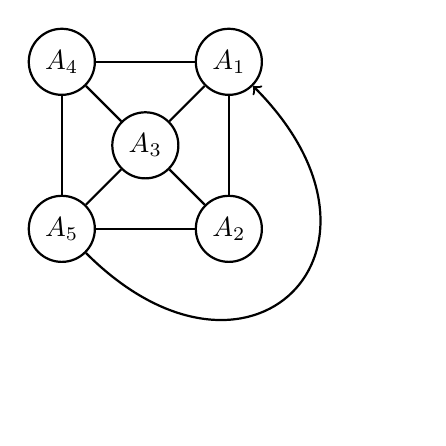
\begin{tikzpicture}[node distance={15mm}, thick, main/.style = {draw, circle}] 
        \node[main] (1) {$A_1$}; 
        \node[main] (3) [below left of=1] {$A_3$}; 
        \node[main] (2) [below right of=3] {$A_2$}; 
        \node[main] (4) [above left of=3] {$A_4$}; 
        \node[main] (5) [below left of=3] {$A_5$}; 
        \draw (1) -- (2); 
        \draw (1) -- (3); 
        \draw (1) -- (4);
        % \draw (1) to [out=135,in=90,looseness=1.5] (5); 
        % \draw (1) to [out=180,in=270,looseness=5] (1); 
        \draw (2) -- (3); 
        \draw (3) -- (4); 
        \draw (5) -- (4);
        \draw (5) -- (3); 
        \draw (2) -- (5);
        \draw[->] (5) to [out=315, in=315, looseness=2.5] (1); 
    \end{tikzpicture} 
    \item Describe the following graph. $$\overline{K}_n$$
    \item [] Since the graph $K_n$ is the graph which has n vertices, n-1 edges and 1 edge between each vertex, $\overline{K}_n$ will be the graph with k vertices with no edges. To take the complement of a graph, you take the connections that the original graph has and remove them while adding connecctions that were not present in the original graph.
    \item Describe the trees produced by the breadth-first search and depth-first search of the complete bipartite
    graph Km,n, starting at a vertex of degree m, where m and n are positive integers. Justify your answers.
    \begin{enumerate}
        \item [Breadth-first:] The graph produced by this algorithm will be starting at the root, visiting any vertices that are adjacent to the root until there are no more to search. Then go visit the first vertex visited from root and repeat.
        \item [Deapth-first:] The graph produced by this algorithm will be starting at the root, visit every vertex adjacent to it and repeat.
        \item[] Refer to attached image for graph drawings.
        % \item [] Example:
        % \begin{tikzpicture}[node distance={15mm}] 
        %     \tikzstyle{every node}=[circle, draw, fill=black, inner sep=0pt, minimum width=4pt]
        %     \node (1) {}; 
        %     \node (2) [right of=1] {}; 
        %     \node (3) [right of=2] {}; 
        %     \node (4) [right of=3] {}; 
        %     \node (5) [right of=4] {}; 
        %     \node (6) [below left of=2] {}; 
        %     \node (7) [below left of=3] {}; 
        %     \draw (1) -- (2); 
        %     \draw (1) -- (6); 
        %     \draw (7) -- (3); 
        %     \draw (6) -- (7); 
        %     \draw (1) -- (3); 
        %     \draw (1) -- (4);
        %     \draw (2) -- (3); 
        %     \draw (3) -- (4); 
        %     \draw (5) -- (4);
        %     \draw (5) -- (3); 
        %     \draw (2) -- (5); 
        % \end{tikzpicture}
    \end{enumerate}   
\end{enumerate}


\end{document}